\section{Experiments}
\label{sec:experiments}

This proposed architecture is based in HED \cite{Xie:2017:HED:3158436.3158453}, RCF \cite{RCF:8100105} and VGG \cite{simonyan2014}. To study the composition of outputs, firstly we used HED approach with side outputs in each stage. Once our problem is not as unbalanced as HED, we decided to use strongly known \textit{categorical\_crossentropy} loss function instead of the custom loss function created in HED and RCF papers.

Also, to merge the side outputs, we used 4 different functions:

\begin{itemize}
 \item \textit{Add} - Sums all predictions provided in each layer to produces only one output;
 
 \item \textit{Average} - Makes the average value of all side outputs;
 
 \item \textit{Maximum} - Takes the result of the most confident output;
 
 \item \textit{Majority} - Takes the prediction values by all outputs and decided for the class that contains the more votes.
\end{itemize}

The fuction \textit{Add} was looking for combine low and high confidence neurons into one single output. \textit{Average} functions aims to combine low confidence neurons with high confidence ones. Also evaluates if all the network is learning the information instead of only part of it. \textit{Max}, for other way, trust only in the most confident value, ignoring low values. This operation does not impply that all network is learning a task, but means that at least one neuron learned. Finally, the \textit{Majority} prediction expecting a kind of consensus of the side outputs.

Since the first tests we clearly saw that \textit{Max} operation was the far best. It was easier to train and produces better results, even without data augmentation. Other operations were difficult to train and requests a carefully set of parameters. The results often are trapped in saddle points and overfitting. This behavior can be seen in Figure \ref{fig:val_accuracy_all}, with the same small learning rate ($1 \times 10^4$) and SGD optimizer. \textit{Max} adapted with less carefully parameters, but also overfits with other optimizers as Adadelta \cite{Adadelta:2012} and Adam \cite{Adam:2014}.

\begin{figure}[ht]
  \centering
  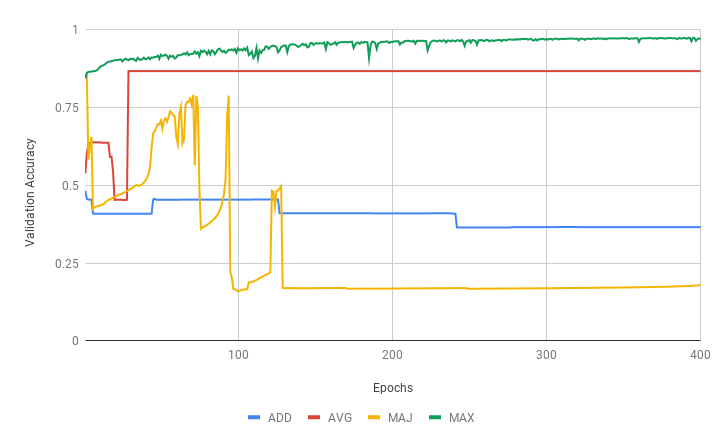
\includegraphics[width=0.48\textwidth]{figures/val_acc_all.png}
  \caption{Validation accuracy}
  \label{fig:val_accuracy_all}
\end{figure}

Once the results were good for \textit{Max} operation, a simple question emerged: ``What happens if we put output all layers of the network?''. Then we put output in all layers and proceeded with \textit{Max} operation. In training evaluation, it was noticed that the network was more stable, and we can set bigger learning rates parameters ($1 \times 10^3$). Also, we can use different optimizers and Nesterov Optimization \cite{Nesterov:1983wy}.

\begin{figure}[ht]
  \centering
  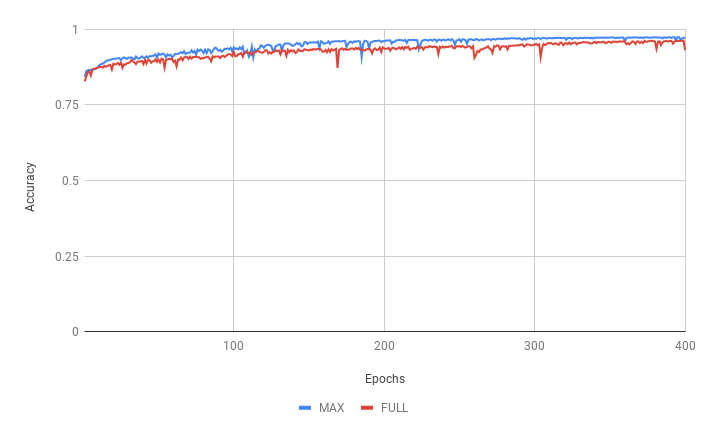
\includegraphics[width=0.48\textwidth]{figures/val_acc.png}
  \caption{Validation accuracy}
  \label{fig:val_accuracy}
\end{figure}

\begin{figure}[ht]
  \centering
  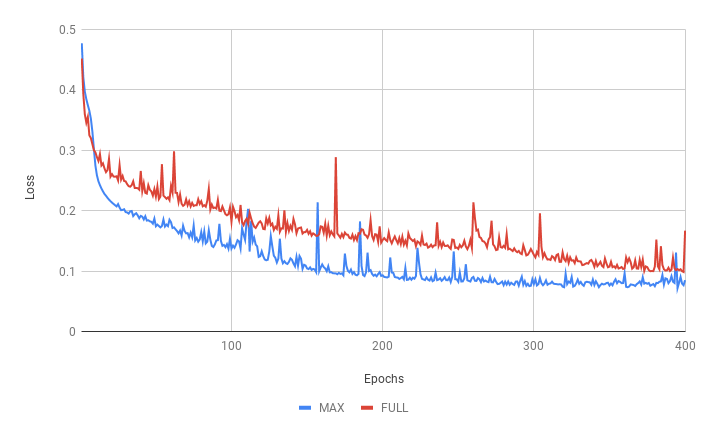
\includegraphics[width=0.48\textwidth]{figures/val_loss.png}
  \caption{Validation loss}
  \label{fig:val_loss}
\end{figure}

\begin{figure}[ht]
  \centering
  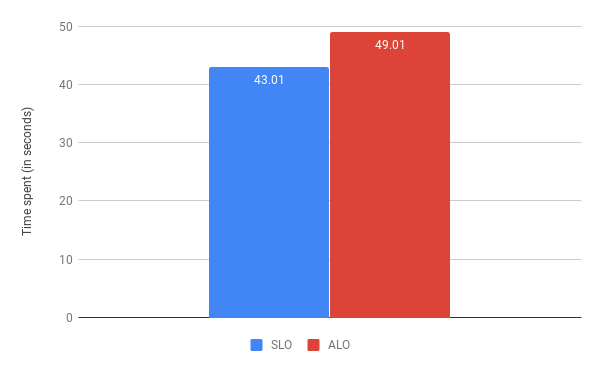
\includegraphics[width=0.48\textwidth]{figures/train_time.png}
  \caption{Average training time}
  \label{fig:train_time}
\end{figure}

\subsection{The Kitti Road/Lane dataset}

KITTI Road/Lane Dataset, part of KITTI Vision Benchmarking Suite, contains  images for road and lane estimation. Consists of 289 training and 290 test images . Ground truth is manually annotated for two different road types: road - road area (the composition of all lanes), and lane (the ego-lane; lane the vehicle is currently driving on) \cite{KITTI}. 

In this paper, we use only the road ground-truths and ignore lane annotations. Some images contains two different ground-truths, one for lane and other for road. Then, we prefer to use road estimation and build only one classifier. Also, it is important to say that ground truth is only available for training set. The test evaluation should be performed using KITTI Server \cite{KITTI}. 

\subsection{Experimental setup}

\subsubsection{Data augmentation and Validation Set}

To increase the number of images in the training set, we made some data augmentation procedures. The techniques we used was pepper noise, horizontal flipping (mirror), contrast and brightness.

These procedures resulted in 1445 images, splited in 1228 samples for training and 217 validate samples (about 15\%).

\subsubsection{Development machine}

The tests were performed in a Intel(R) Core(TM) i7-8700 CPU @ 3.20GHz with 32 GB RAM and a GeForce GTX 1080 8GB GPU. The tests were developed using Keras \cite{chollet2015keras} with Tensorflow \cite{tensorflow2015-whitepaper} in a Ubuntu 16.04 OS. The setup under Anaconda environment is public available in \url{https://github.com/falreis/segmentation-eval}.

\subsection{Results}

\begin{table}
  \begin{tabular}{{c}{c}{c}{c}{c}{c}{c}}
  
  \multicolumn{7}{l}{Stage Layer Outputs - Without Matematical Morfology} \\
  \hline 
    Category & MaxF & AP & PRE & REC & FPR & FNR \\
  \hline
    \textit{um\_road} & 96.92\% & 87.36\% & 94.47\% & 99.49\% & 1.13\% & 0.51\% \\
    \textit{umm\_road} & 97.57\% & 89.44\% & 96.05\% & 99.15\% & 1.24\% & 0.85\% \\
    \textit{uu\_road} & 95.16\% & 85.73\% & 92.94\% & 97.49\% & 1.16\% & 2.51\% \\
  \hline
  \multicolumn{7}{c}{} \\
  
  \multicolumn{7}{l}{Stage Layer Outputs - With Matematical Morfology} \\
  \hline 	
    Category & MaxF & AP & PRE & REC & FPR & FNR \\
  \hline
    \textit{um\_road} & 97.01\% & 87.68\% & 94.83\% & 99.30\% & 1.05\% & 0.70\% \\
    \textit{umm\_road} & 97.61\% & 89.67\% & 96.30\% & 98.97\% & 1.16\% & 1.03\% \\
    \textit{uu\_road} & 95.42\% & 86.48\% & 93.77\% & 97.13\% & 1.01\% & 2.87\% \\
  \hline
  \multicolumn{7}{c}{} \\
  
  \multicolumn{7}{l}{All Layers Outputs - Without Matematical Morfology} \\
  \hline 	
    Category & MaxF & AP & PRE & REC & FPR & FNR \\
  \hline
    \textit{um\_road} & 96.39\% & 86.81\% & 93.87\% & 99.05\% & 1.25\% & 0.95\% \\
    \textit{umm\_road} & 97.05\% & 88.83\% & 95.37\% & 98.78\% & 1.46\% & 1.22\% \\
    \textit{uu\_road} & 94.70\% & 84.87\% & 92.00\% & 97.56\% & 1.33\% & 2.44\% \\
  \hline
  \multicolumn{7}{c}{} \\
  
  \multicolumn{7}{l}{All Layers Outputs - With Matematical Morfology} \\
  \hline 	
    Category & MaxF & AP & PRE & REC & FPR & FNR \\
  \hline
    \textit{um\_road} & 96.65\% & 87.51\% & 94.64\% & 98.74\% & 1.08\% & 1.26\% \\
    \textit{umm\_road} & 97.21\% & 89.31\% & 95.90\% & 98.56\% & 1.29\% & 1.44\% \\
    \textit{uu\_road} & 95.20\% & 86.15\% & 93.40\% & 97.08\% & 1.08\% & 2.92\% \\
  \hline
  
  \end{tabular}
  \caption{KITTI benchmark evaluation results for in each category \protect\footnotemark}
  \label{table:max_without_morf}
\end{table}

\footnotetext{Table abbreviations: \textit{MaxF}: Maximum F1-measure, \textit{AP}: Average precision, \textit{PRE}: Precision, \textit{REC}: Recall, \textit{FPR}: False Positive Rate, \textit{FNR}: False Negative Rate}

\begin{comment}
HED
Closing for i in range(3, 8, 1):


\end{comment}

\subsection{Qualitative analysis}
